\documentclass{article}
\usepackage[utf8]{inputenc}
\usepackage{graphicx}
\usepackage{amsmath}
\usepackage{listings}
\usepackage[norsk]{babel}

\title{Oblig 1b: Analyse av Terningdropp}
\author{Ditt Navn}
\date{Innleveringsdato}

\begin{document}

\maketitle

\section{Introduksjon}
Kort beskrivelse av oppgavens mål og de metoder som brukes.

\section{Datainnsamling og Analyse}

\subsection{2a: Regresjonsanalyse for de Første 5 Målingene}
\begin{lstlisting}[language=R]
lm_first5 <- lm(Lengde ~ Dropp, data=df[1:5, ])
summary(lm_first5)
\end{lstlisting}
\textbf{Regresjonslinje (2a):} Inkluder resultatet fra R og sammenlign med manuell beregning.

\subsection{Question 2b: Scatter Plot of Data Points}
\textit{Scatter plot of the Dropp vs Lengde data (placeholder image).}
\begin{figure}[h]
    \centering
    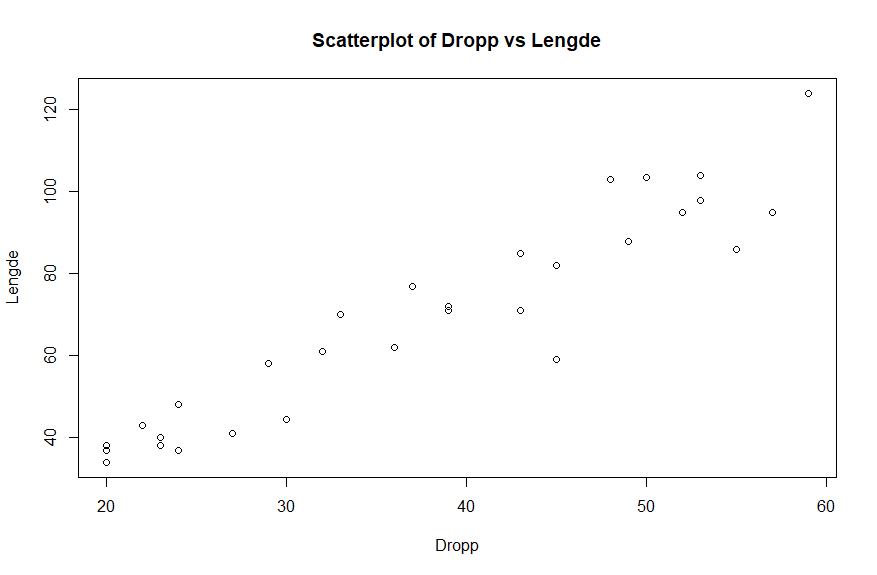
\includegraphics[width=0.8\textwidth]{Rplot03.png}
    \caption{Scatter plot of Dropp vs Lengde}
\end{figure}

\subsection{Question 2c: Regression Line Plot}
\textit{Scatter plot with regression line (placeholder image).}
\begin{figure}[h]
    \centering
    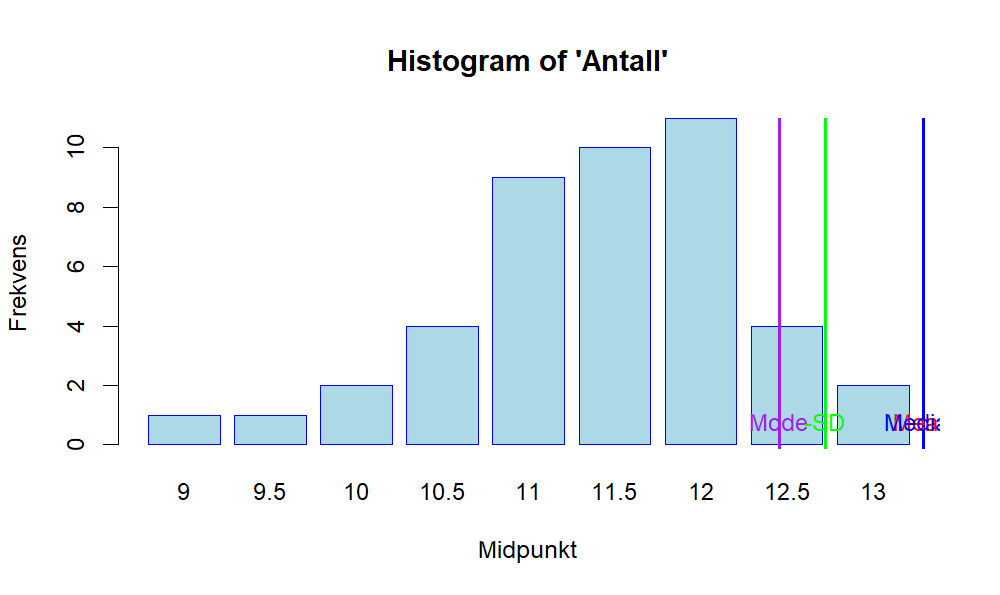
\includegraphics[width=0.8\textwidth]{Rplot02.png}
    \caption{Scatter plot with regression line}
\end{figure}

\subsection{2c: Regresjonsanalyse for Hele Datasettet}
\begin{lstlisting}[language=R]
lm_full <- lm(Lengde ~ Dropp, data=df)
\end{lstlisting}

\subsection{2d: Spreddiagram av Data}
\begin{figure}[h]
    \centering
    \includegraphics[width=0.8\textwidth]{scatterplot.png}
    \caption{Spreddiagram av Dropp mot Lengde (2d)}
\end{figure}

\subsection{2e: Spreddiagram med Regresjonslinje}
\begin{figure}[h]
    \centering
    \includegraphics[width=0.8\textwidth]{regression_plot.png}
    \caption{Spreddiagram med regresjonslinje (2e)}
\end{figure}

\subsection{2g: Sum av Kvadrerte Residualer (SSe)}
\begin{lstlisting}[language=R]
ssr_first5 <- sum(residuals(lm_first5)^2)
ssr_full <- sum(residuals(lm_full)^2)
\end{lstlisting}
\textbf{SSR (2g):} SSR for de første 5 målingene: \[ <ssr_first5> \]
SSR for hele datasettet: \[ <ssr_full> \]

\subsection{2h: Standardfeil (se)}
\begin{lstlisting}[language=R]
se_first5 <- sqrt(ssr_first5 / lm_first5$df.residual)
se_full <- sqrt(ssr_full / lm_full$df.residual)
\end{lstlisting}
\textbf{Standardfeil (2h):} SE for de første 5 målingene: \[ <se_first5> \]
SE for hele datasettet: \[ <se_full> \]

\subsection{2i: Lagring av Arbeid}
Beskrivelse av hvordan arbeidet ble lagret og dokumentert.

\section{Konklusjon}
Oppsummer dine funn og observasjoner fra oppgaven.

\end{document}
